% !TeX document-id = {54177b55-cdde-488b-90fe-107922d59049}
\documentclass[12pt]{article}

\usepackage{a4} 
\usepackage{amsmath}
\usepackage{amssymb}
\usepackage[]{xcolor}
\usepackage{graphicx}
\usepackage[colorlinks,urlcolor=blue,linkcolor=blue,citecolor=hotpink]{hyperref}
\usepackage{booktabs}
\usepackage{rotating}
\usepackage{caption}
\usepackage[british]{babel}
\usepackage[linesnumbered, ruled]{algorithm2e}
\usepackage{epstopdf}
\usepackage{mathtools} % for :=
\usepackage{subfig}
\usepackage[most, minted]{tcolorbox}
\usepackage{mdwlist}
\tcbuselibrary{listings}
%\usepackage[cache=false]{minted} % Need cache=false or leads to funny bug.
% !TeX TXS-program:compile = txs:///pdflatex/[--shell-escape]

\newtcblisting{myminted}{%
	listing engine=minted,
	minted language=python,
	listing only,
	breakable,
	enhanced,
	minted options = {
		linenos, 
		breaklines=true, 
		breakanywhere, 
		fontsize=\footnotesize, 
		numbersep=2mm,
		tabsize=2
	},
	overlay={%
		\begin{tcbclipinterior}
			\fill[gray!25] (frame.south west) rectangle ([xshift=4mm]frame.north west);
		\end{tcbclipinterior}
	}   
}
\BeforeBeginEnvironment{minted}{\begin{tcolorbox}[breakable, enhanced]}%
	\AfterEndEnvironment{minted}{\end{tcolorbox}}%


\graphicspath{{images/}}

\title{Critical path estimation in heterogeneous scheduling heuristics} % Think of a better title...
\author{Thomas McSweeney%
	\thanks{%
		School of Mathematics,
		University of Manchester,
		Manchester, M13 9PL, England
		(\texttt{thomas.mcsweeney@postgrad.manchester.ac.uk}).
	}
}
\date{\today}

%%%%%%%%%%%%%%%%%%%%%%%%%%%%%%%%%
\def\R{\mathbb{R}}
\def\C{\mathbb{C}}
\def\P{\mathbb{P}}
\def\E{\mathbb{E}}
\def\nbyn{n \times n}
\def\mbyn{m \times n}
\def\l{\lambda}
\def\norm#1{\|#1\|}      
\def\normi#1{\|#1\|_1}
\def\normo#1{\|#1\|_{\infty}}
\def\Chat{\widehat{C}}
\def\e{eigenvalue}
\DeclareMathOperator*{\argmax}{arg\,max}
\DeclareMathOperator*{\argmin}{arg\,min}

% \DeclareMathOperator{\diag}{diag}   % Requires amsmath.
\def\diag{\mathop{\mathrm{diag}}}     % If not using amsmath.
\def\trace{\mathop{\mathrm{trace}}}   % If not using amsmath.

\def\At{\widetilde{A}}
\def\normt#1{\|#1\|_2}

% Set up lemma environment and its numbering.
\newtheorem{lemma}{Lemma}[section]

\def\proof{\par{\bf Proof}. \ignorespaces}
\def\qedsymbol{\vbox{\hrule\hbox{%
			\vrule height1.3ex\hskip0.8ex\vrule}\hrule}}
\def\endproof{\qquad\qedsymbol\medskip\par}

\newtheorem{theorem}{Theorem}
\newtheorem{prop}[theorem]{Proposition}

\allowdisplaybreaks[1]

%%%%%%%%%%%%%%%%%%%%%%%%%%%%%%%%%%%%%%%%%%%%%%%%%%%%%%%%%%%%%%%%%%%%%%%%%%%%
% For fine-tuning spacing in \sqrt etc=.  From \cite[p.~155]{knut99}.
% In math mode, @ will act as a macro that adds 1 unit of space.
% By comparison, \, skips 3mu.

\mathcode`@="8000 % Make @ behave as per catcode 13 (active).  TeXbook p. 155.
{\catcode`\@=\active\gdef@{\mkern1mu}}
%%%%%%%%%%%%%%%%%%%%%%%%%%%%%%%%%%%%%%%%%%%%%%%%

%%%%%%%%%%%%%%%%%%%%%%%%%%%%%%%%%%%%%%%%%%%%%%%%%%%%%%%%%%%%%%%%%%%%%%%%%%%%
\newcounter{mylineno}
\makeatletter
\let\oldtabcr\@tabcr
\def\nonumberbreak{\oldtabcr\hspace{3.5pt}}
\def\mynewline{\refstepcounter{mylineno}%
	\llap{\footnotesize\arabic{mylineno}\hspace{5pt}}%
}
\def\lineref#1{\footnotesize\ref{#1}}
% Next macro adapted from latex.ltx
\gdef\@tabcr{\@stopline \@ifstar{\penalty%
		\@M \@xtabcr}\@xtabcr\mynewline}
\def\myvspace#1{\oldtabcr[#1]\mynewline}
\newenvironment{code}{%
	% Swap `:' and `colon'...
	\mathcode`\:="603A  % TeXbook pp 134, 154, 359 (top)
	% For original colon     \mathcode`\:="303A  % TeXbook p 344
	\def\colon{\mathchar"303A}
	\setcounter{mylineno}{0}
	\par
	\upshape
	\begin{list} % To give indentation
		{} {\leftmargin = 1cm}
		\item[]
		\begin{tabbing}
			
			% Default tab stops
			\hspace*{.3in} \= \hspace*{.3in} \=
			\hspace*{.3in} \= \hspace*{.3in} \= \kill
			\mynewline
		}{\end{tabbing}\end{list}}
\makeatother


\addto\captionsbritish{	\renewcommand{\bibname}%
	{References}%TODO: make sure reference style is consistent.
}

\definecolor{hotpink}{rgb}{0.9,0,0.5}

\begin{document}
	\maketitle 	


\section{Introduction}
\label{sect.intro}

%Before describing HEFT, we first introduce the concept of the {\em critical path}. The name comes from project management, where it is defined as the longest sequence of activities that must be done in order to complete a project \cite{kel59,kel61}; for a task graph, the critical path is the longest (costliest) path through it. This is useful because, if we assume sufficient parallelism, then the time it takes to execute the tasks on the critical path of a DAG therefore gives a lower bound on the makespan of any schedule. A natural approach in a listing heuristic then is to prioritize all tasks according to the length of the critical path from that task to the end; the idea being that tasks with the greatest downward path length contribute most towards the makespan and should therefore be processed as soon as possible. This approach has a long and successful history in scheduling for homogeneous processors \cite{cof72} but it isn't clear how it should be defined for heterogeneous ones, when all DAG costs can take multiple values and there are many possible critical paths (see Chapter \ref{chap.critical_path_estimation}).

Recall from Chapter X that the {\em Heterogeneous Earliest Finish Time} (HEFT) heuristic prioritizes all tasks $t_i$, $i = 1, \dots, n$, by recursively computing a corresponding sequence of numbers $u_i$ which are intended to represent {\em critical path} lengths from each task to the end. However, as noted previously, the concept of the {\em critical path} is not clearly defined: DAG weights are not fixed at this stage so there are multiple ways we could define a {\em longest} (i.e., {\em costliest}) path. Consider for example the simple DAG shown in Figure \ref{plot.simple_example}, where the labels represent all the possible weights each task/edge may take on a two-processor target platform; more specifically, the labels $(W_i^1, W_i^2)$ near the nodes represent the computation costs on processors $P1$ and $P2$, respectively, while the edge labels $(0 = W_{ik}^{11} = W_{ik}^{22}, W_{ik}^{12}, W_{ik}^{21})$ represent the possible communication costs. What is the longest path through this graph? 

\begin{figure}
	\centering	
	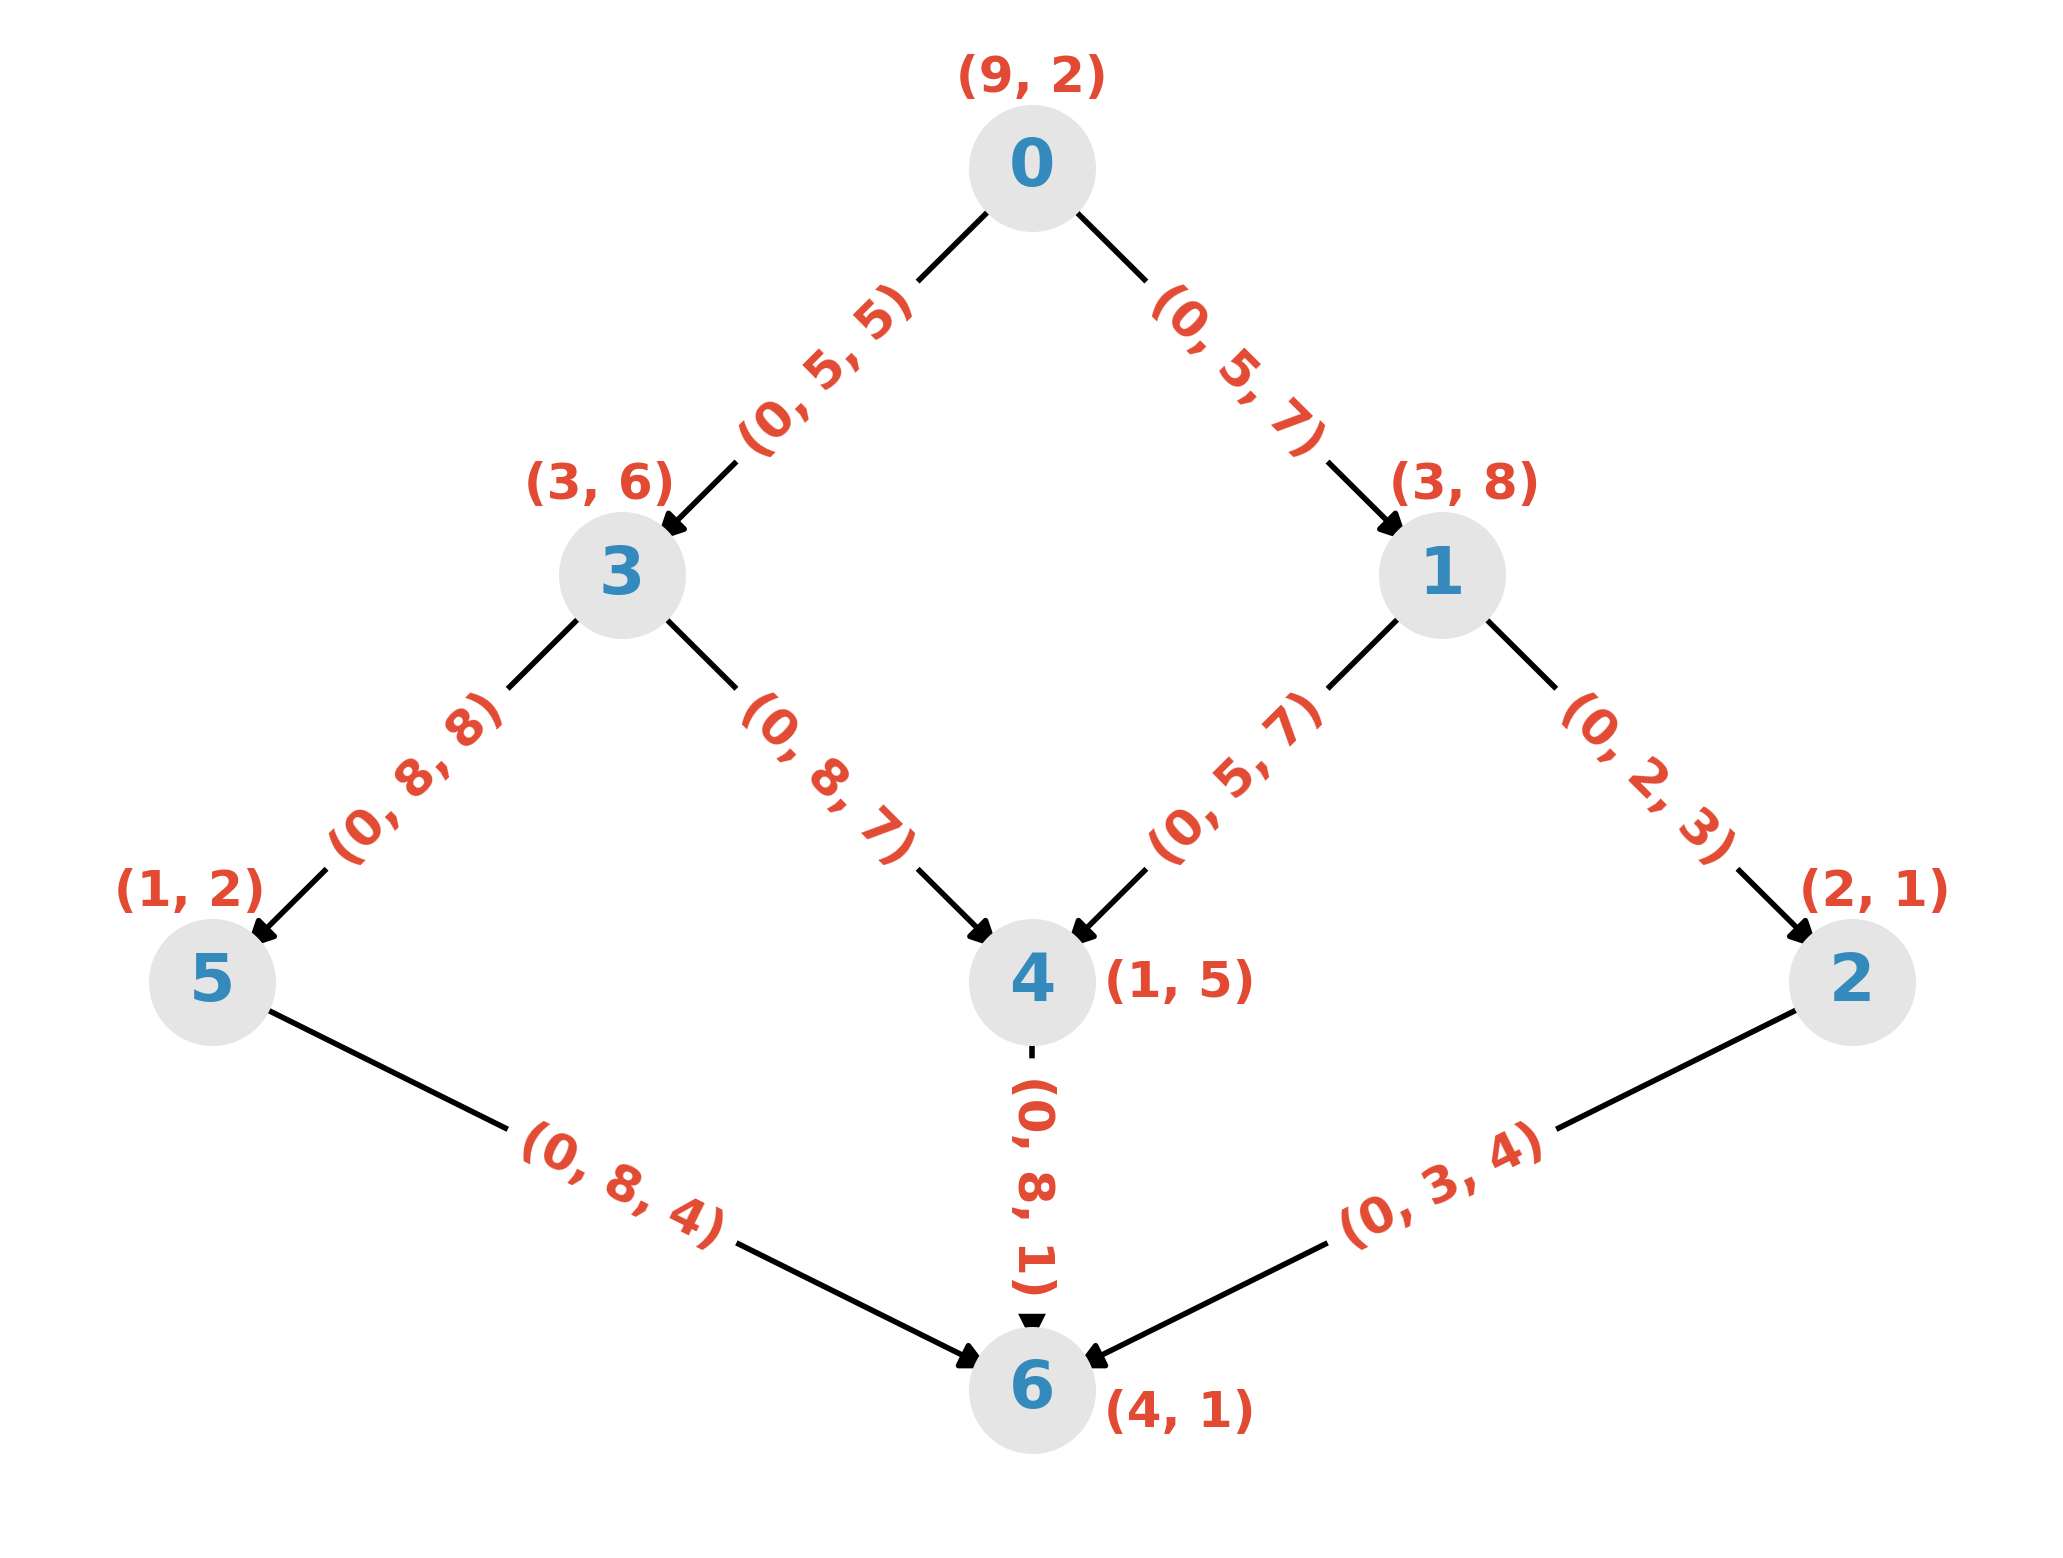
\includegraphics[scale=0.7]{simple_graph.png}
	\caption{Simple task graph with costs on a two-processor target platform.}	
	\label{plot.simple_example}
\end{figure}

Clearly there are multiple possible ways this can be defined. The HEFT approach, as described in previous chapters, is to use mean values over all sets of possible task and edge costs to transform the DAG into a fixed-cost version, as in Figure Y, and then compute the critical path lengths in a standard dynamic programming way to find the task ranks. For the simple graph, we find that $u_4 = 5$, $u_3 = 19/2$, $u_2 = 21/2$ and $u_1 = 16$. Now, it should be clear that the optimal schedule for the example graph is to simply schedule all tasks on processor $P1$, which gives us a schedule of length $6$. Although HEFT finds the optimal schedule, the $u_i$ values are not bounds on the schedule makespan... Conceptually, the HEFT critical path isn't a lower bound on any schedule makespan but a lower bound on what the schedule is likely to be...

Given this ambiguity, alternative ways to definite the critical path in HEFT have been considered before, most notably by Zhao and Sakellariou \cite{zhao03}, who empirically compared the performance of HEFT when averages other than the mean (e.g., median, maximum, minimum) are used to compute upward (or downward) ranks. Their conclusions were that using the mean is not clearly superior to other averages, although none of the other options were consistently better. Indeed, perhaps the biggest takeaway from their investigation was that HEFT is very sensitive to how priorities are computed, with significant variation being seen for different graphs and target platforms. In this chapter we undertake a similar investigation with the aim of establishing if there are choices which do consistently outperform the standard HEFT task ranking phase.   

This will be an empirically-driven study, as is common in this area. To facilitate this investigation we created a software package that simulates heterogeneous scheduling problems, much like that described in the previous chapter, although not restricted to accelerated target platforms. As before, the ({\tt Python}) source code for this simulator can be found on Github\footnote{\href{https://github.com/mcsweeney90/critical-path-estimation}{{\tt \small https://github.com/mcsweeney90/critical-path-estimation}}} and all of the results presented here can be re-run from scripts contained therein. 

% TODO: mention that only giving equations etc for u_i but can analagously define d_i. 

\section{Optimistic bounds}
\label{sect.optimistic}

Functionally, the critical path is used in HEFT as a lower bound on the makespan, so that minimizing the critical path gives us the most scope to minimize the makespan (assuming we make good use of our parallel resources). With this in mind, there are many different ways we can define the critical path so that it gives a lower bound on the makespan of any possible schedule. The most straightforward approach would be to just set all weights to their minimal values but a tighter bound can be computed in the following manner. First, define $u_i^a$ for all tasks $t_i$ and processors $p_a$ to be the critical path length from $t_i$ to the end (inclusive), assuming that it is scheduled on processor $p_a$. These values can easily be computed recursively by setting $u_i^a = W_i^a \; \forall a$ for all exit tasks then moving up the DAG and setting 
\begin{align}
u_i^a &= W_i^a + \max_{k \in S_i} \bigg( \min_{b = 1, \dots, q} \big( u_k^b + W_{ik}^{ab} \big)  \bigg) \quad \forall a \label{eq.opt_uia} 
\end{align}
for all other tasks. Then for each $i = 1, \dots, n$,
\begin{align}
u_i &= \min_{a = 1, \dots, q}u_i^a \label{eq.opt_ui} 
\end{align}
gives a true lower bound on the remaining cost of any schedule once the execution of task $t_i$ begins. These $u_i$ values could be useful as alternative task priorities in HEFT, especially since the cost of computing all of the $u_i^a$ in this manner is only $O(m + n) \approx O(n^2)$ so in particular is no more expensive than the usual HEFT prioritization phase. Of course, it should be emphasized here that there is absolutely no mathematically valid reason to suppose that doing so will actually lead to superior performance. Still, it seems worthwhile to investigate this empirically using our simulator, which we duly do in Section \ref{sect.experimental_rankings}. 

Although taking the minimum over the set of processors as in \eqref{eq.opt_ui} is the only choice that gives a true lower bound, we could use any other average over the set of processors, such as the mean or maximum, in order to compute task priorities. Since we also consider those two alternatives in Section \ref{sect.experimental_rankings}, we refer to the ranking phase defined by using the minimum, maximum and mean as OPT-MIN, OPT-MAX and OPT-MEAN respectively.    

(Note that the optimistic critical path defined here is extremely similar to the optimistic cost used in the PEFT heuristic; this will be discussed further in Section \ref{sect.processor_selection}.)


\section{Alternative rankings}
\label{sect.alt_rankings}

In this section we propose a family of alternative task ranking phases in HEFT based on the following interpretation of the standard ranking phase. First, note that by using average values over all sets of possible task and edge costs, HEFT is implicitly assuming that any member of any set is just as likely to be incurred as any other; conceptually, HEFT is attempting to account for the uncertainty of the processor selection phase by assuming that for any given task all processors are equally likely to ultimately be chosen. So, effectively, at the prioritization phase HEFT views the node and edge weights as discrete random variables (RVs) with associated probability mass functions (pmfs) given by the aforementioned assumption. More precisely, let $m_i$ be the pmf corresponding to the task weight variable $w_i$ and $m_{ik}$ that for the edge weight $w_{ik}$, then  
\begin{align*}
m_i(W_i^a) \coloneqq \P[w_i = W_i^a] = \frac{1}{n_p} \quad \forall a
\end{align*}
and   
\begin{align*}
m_{ik}(W_{ik}^{ab}) &= m_i(W_i^a) \cdot m_k(W_k^b) \\
&= \frac{1}{n_p^2} \quad \forall a, b.
\end{align*}
Note that the expected values of the node and edge weights are therefore given by
\begin{align}
\E[w_i] &= \sum_{\ell \in L_i} \ell m_i(\ell) = \frac{1}{n_p} \sum_{a} W_i^a \label{eq.expected_node}\\
\E[w_{ik}] &= \sum_{\ell \in L_{ik}} \ell m_{ik}(\ell) = \frac{1}{n_p^2} \sum_{a, b} W_{ik}^{ab} \label{eq.expected_edge}.
\end{align}
In particular, this means that $\E[w_i] = \overline{w_i}$ and $\E[w_{ik}] = \overline{w_{ik}}$ so that the computation of the upward ranks $u_i$ can instead be done by setting $u_i = \E[w_i]$ for all exit tasks, then moving up the DAG and recursively computing
\begin{align}
u_i = \E[w_i] + \max_{k \in S_i} \big( u_k + \E[w_{ik}] \big) \label{eq.ur_expectation}
\end{align}
for all other tasks.

To sum up, since all possible node and edge weights are known but their actual values at runtime aren't (at least without restricting the processor selection phase), HEFT estimates critical path lengths from all tasks in a task graph $G$ through a two-step process:
\begin{enumerate}
	\item An associated graph $G_s$---referred to as {\em stochastic} because all of its weights are RVs---is implicitly constructed with node and edge pmfs $m_i$ and $m_{ik}$ as defined above.   
	\item The numbers $u_i$ are recursively computed for all tasks in $G_s$ using \eqref{eq.ur_expectation}, and taken as the critical path lengths from the corresponding tasks in $G$.      
\end{enumerate}
In the following two sections, we propose modifications of both steps so as to obtain different critical path estimates that may be used as task ranks in HEFT. The performance of these will then be evaluated through extensive numerical simulations in Section \ref{sect.experimental_rankings}.

\subsection{Sharper bounds on the critical path of $G_s$}
\label{subsect.sharper_bounds}

A natural question arises from the interpretation outlined in the previous section: what is the relationship between the sequence of numbers $u_i$ and the critical path of the stochastic graph $G_s$? Computing the distribution of the critical path length, or even just the moments, for a general stochastic DAG is known to be a difficult problem and is discussed in much more detail in Chapter X. However, suffice it to say here, it has long been known in the context of {\em Program Evaluation and Review Technique} (PERT) network analysis that the numbers $u_i$ are in fact {\em lower bounds} on the expected value of the critical path lengths of the stochastic DAG. This result dates back at least as far as Fulkerson \cite{fulk62}, who referred to it as already being widely-known and gave a simple proof. Furthermore, he also showed how a sequences of numbers which give tighter bounds can easily be constructed.

\subsubsection{Fulkerson's bound}
\label{subsubsect.fulkerson}

First we explain how the DAG as shown in Figure \ref{plot.cp_example} can be expressed in an equivalent formulation with only edge weights. This step is not strictly necessary but simply makes the elucidation cleaner; we should emphasize that all of the following still holds, with only minor adjustments, if this is not done.

Suppose $(t_i, t_k)$ is any edge of the DAG and its cost $w_{ik}$ represents the computation cost of the parent task $t_i$ plus the communication cost of the edge, unless $t_k$ is an exit task, in which case the edge cost also includes the computation cost of $t_k$. Let $\tilde{c}_{ik} = c_i + \delta_kc_k$ where $\delta_{k} = 1$ if $t_k$ is an exit task and $0$ otherwise. Likewise, let $\tilde{g}_{ik} = g_i + \delta_{k}g_k$. For $s \in \{ c, g \}$, define   
\begin{align*}
\tilde{C}_{ik}^s = C_{ik}^s + \tilde{c}_{ik} \quad \text{and} \quad \tilde{G}_{ik}^s = G_{ik}^s + \tilde{g}_{ik}.
\end{align*}
Then the edge can take one of six possible values, as illustrated in Figure \ref{plot.aoa_labels}, so that the simple DAG from Figure \ref{plot.cp_example} can be represented instead as in Figure \ref{plot.aoa_example_graph}. Let $\tilde{L}_{ik} = \{ \tilde{c}_{ik}, \tilde{C}_{ik}^c, \tilde{C}_{ik}^g, \tilde{g}_{ik}, \tilde{G}_{ik}^g, \tilde{G}_{ik}^c \}$ be the set of all possible costs the edge may represent.

To compute the upward ranks of all tasks, the estimated edge pmfs $m_{ik}$ need to be replaced by very similar functions $\tilde{m}_{ik}$ defined by
\begin{align*}
\tilde{m}_{ik}(\tilde{c}_{ik}) = \frac{n_c}{n_p^2}, &\qquad \tilde{m}_{ik}(\tilde{C}_{ik}^c) = \frac{n_c(n_c - 1)}{n_p^2}, \\
\tilde{w}_{ik} (\tilde{g}_{ik}) = \frac{n_g}{n_p^2}, &\qquad \tilde{m}_{ik}(\tilde{G}_{ik}^g) = \frac{n_g(n_g - 1)}{n_p^2},\\
\qquad \tilde{m}_{ik}( \tilde{C}_{ik}^g) &= \tilde{m}_{ik} (\tilde{G}_{ik}^c) = \frac{n_cn_g}{n_p^2}.
\end{align*}
The ranks themselves are then given by working up from the leaves of the DAG and recursively computing 
\begin{equation}
\tilde{u}_i =\left\{
\begin{array}{@{}ll@{}}
0, \quad  \text{if $t_i$ is an exit task,} \\
\max_{k \in S_i} \{ \tilde{u}_k + \E[w_{ik}] \},  \quad \text{ otherwise},
\end{array}\right.
\label{eq.ur_edges_only}
\end{equation}
where the expectation is computed using the pmfs $\tilde{m}_{ik}$. It can readily be verified that this sequence of numbers is identical to the $u_i$, with the exception of those corresponding to exit tasks which are now equal to zero. Note that here we have used the default HEFT pmfs $m$ as the basis for $\tilde{m}$, when we could just as easily have used the {\em biased} version $\hat{m}$ defined in Section \ref{subsect.biasing}. We will use the default throughout this section but the alternative is also considered when results are presented in Section \ref{subsect.prioritization_results}. 

Let $W_i \coloneqq \{ w_{ik} \}_{k \in S_i}$ be the set of all the weight RVs corresponding to edges which connect task $t_i$ to its children. Assume that all tasks are indexed in a topological order, so that in particular if $t_k$ is a child of $t_i$ then $i > k$, and define 
\begin{align*}
Z_i \coloneqq W_i \cup \{ W_k \}_{k \in S_i}.
\end{align*}
Let $R_i$ be the set of all possible {\em realizations} of the RVs in $Z_i$ and suppose that $z_i \in R_i$ can be expressed in the form 
\begin{align*}
z_i = z_i^i \cup \{ z_i^k \}_{k \in S_i}.
\end{align*}
where $z_i^k$ contains the realizations of the RVs in $W_k$. Given a realization $z_i \in R_i$, let $\ell(z_i)$ be the critical path length from task $t_i$ to the end. Define $e_i$ to be the expected downward critical path length from, and including, task $t_i$. Then by definition we have
\begin{align}
e_i &= \sum_{z_i \in R_i} \P[Z_i = z_i] \ell(z_i). \label{eq.expected_cp}
\end{align}
By taking average values over all processors for each task weight, HEFT effectively assumes that they are all independent of one another, although of course this may not in fact be the case. Likewise the edge weights are also implicitly regarded as being independent both of each other and the task weights, which is definitely not true since they are entirely determined once the task weights $w_i$ are realized.  Disregarding this modeling inaccuracy for the moment, for the edge weight-only version of the stochastic DAG that we are using here, all of the RVs $w_{ik} \in W_i$ incorporate the task weight RV $w_i$ so that they are no longer independent of one another---but they are still assumed to be independent of the edge weights in the other sets $W_j$, $j \neq i$. In particular, this implies that 
\begin{align}
\P[Z_i = z_i] = \P[W_i = z_i^i] \prod_{k \in S_i} \P[W_k = z_i^k]. \label{eq.independence_assumption}
\end{align}  
With this we can rewrite equation \eqref{eq.expected_cp} as
\begin{align}
e_i &= \sum_{z_i \in R_i} \P[Z_i = z_i] \ell(z_i) \nonumber \\
&= \sum_{z_i^i} \sum_{\substack{z_k \in R_k, \\ k \in S_i}} \P[W_i = z_i^i] \P[Z_{k} = z_{k}] \max_{k \in S_i} \{ \ell(z_{k}) + z_{ik} \}, 
\end{align}
where $z_{ik}$ is the realization of the edge weight RV $w_{ik}$ defined by the set of realizations $z_k$. It is now relatively straightforward to show that the identity $\tilde{u}_i \leq e_i$ (and therefore $u_i \leq f_i$) holds for all tasks $t_i$ by manipulating this expression; the reader is directed to Fulkerson's original paper for full details \cite{fulk62}. Moreover, suppose we define a sequence of numbers by $f_i = 0$, if $t_i$ is an exit task, and
\begin{align}
f_i &= \sum_{z_i \in R_i} \P[Z_i = z_i] \max_{k \in S_i} \{ f_k + z_{ik} \} \nonumber \\
&= \sum_{z_i^i} \sum_{\substack{z_k \in R_k, \\ k \in S_i}} \P[W_i = z_i^i] \P[Z_{k} = z_{k}] \max_{k \in S_i} \{ f_k + z_{ik} \}, \label{eq.f_fulkerson}
\end{align}
for all other tasks. Then Fulkerson showed that the identity $u_i \leq f_i \leq e_i$ also holds for all tasks---i.e, the $f_i$ give a tighter bound on the expected value of the critical path lengths.

Although the bound is tighter, for each of the $f_i$ we need to do an awful lot of work: suppose $t_i$ has $K$ children, then for any one of them $t_k$ we need to do $O(|\tilde{L}_{ik}|)$ operations, i.e., $O(|\tilde{L}_{ik}|^K)$ in total. Even in this simple example for which $|\tilde{L}_{ik}| \equiv 6$ this quickly becomes impractical, as suggested by our (deliberately) tedious breakdown of the calculations above. In more general heterogeneous environments, $|\tilde{L}_{ik}|$ can be $O(p^2)$ so computing the $f_i$ is even more daunting. Fortunately, a much more efficient method of computing the $f_i$ was given by Clingen \cite{cling64} in the context of extending Fulkerson's method to the case where edge weights are modeled as continuous random variables, although here we follow the slightly more compact notation of Elmaghraby \cite{elmaghraby67}. 

It is well-known that the cumulative probability mass function of the maximum of a finite set of discrete RVs is equal to the product of the individual cumulative pmfs of the RVs. Let $M_{ik}$ be the cumulative pmf along edge $(t_i, t_k)$, so that $M_{ik}(x) = \P[\tilde{w}_{ik} \leq x]$. Define the related function $M_{ik}^{*}(x) = \P[\tilde{w}_{ik} < x]$. Let $Z_i$ be the set of all {\em unique} possible values of $f_k + \tilde{w}_{ik}$, for $k \in S_i$, and let $z$ run over all elements of $Z_i$. For $i = 1, \dots, n$, define 
\begin{align}
\alpha_i &= \max_{k \in S_i}(f_k + \min(\tilde{L}_{ik})).
\end{align}
Then, with the cost independence assumptions we have already made, we can rewrite equation \eqref{eq.f_fulkerson} as 
\begin{align}
f_i &= \sum_{z \geq \alpha_i} z \bigg( \prod_{k \in S_i} M_{ik}(z - f_k) - \prod_{k \in S_i} M_{ik}^{*}(z - f_k) \bigg). \label{eq.f_clingen}
\end{align}
A complete description of a practical procedure for computing the Fulkerson numbers $f_i$ is given in Algorithm \ref{alg.fulkerson}. At first blush this may not appear to be any simpler than before but, crucially, the number of  operations required to compute each of the $f_i$ is $O(|\tilde{L}_{ik}| \cdot K)$, where $K$ is the number of child tasks, rather than the first term being exponential in the second as before. Of course, this procedure is {\em still} more expensive than computing $\tilde{u}_i$ using \eqref{eq.ur_edges_only}, but in our experience it was practical even for large, dense DAGs and target platforms comprising numerous processing resources (albeit so far we have only consider accelerated platforms that follow the model described in Chapter \ref{chap.static_accelerated}).
\begin{algorithm}	
	
	\For{$i = n, \dots, 1$}
	{	
		$f_i = 0$, $\alpha_i = 0$, $Z_i = \{\}$
		
		\For{$k \in S_i$}
		{
			$\ell_m = \infty$
			
			\For{$\ell \in \tilde{L}_{ik}$}
			{
				$\ell_m \leftarrow \min(\ell_m, \ell)$
				
				\If{$f_k + \ell \notin Z_i$}{$Z_i \leftarrow Z_i \cup \{f_k + \ell \}$}
			}
			
			$\alpha_i \leftarrow \max(\alpha_i, f_k + \ell_m)$
		}
		
		
		\For{$z \in Z_i$}
		{
			\If{$z \geq \alpha_i$}
			{
				$g = 1$, $q = 1$
				
				\For{$k \in S_i$}
				{
					$g \leftarrow g \times M_{ik}(z - f_k)$
					
					$q \leftarrow q \times M_{ik}^{*}(z - f_k)$
				}
				
				$f_i \leftarrow f_i + z \times (g - q)$				
			}
		}		
	}	
	\caption{Computing the Fulkerson numbers using Clingen's method.}
	\label{alg.fulkerson}
\end{algorithm} 

Once all of the $f_i$ have been computed, they can be taken as alternative task ranks in HEFT (or any listing heuristic). However, it should be emphasized here that although the $f_i$ give tighter bounds on the critical path lengths of the stochastic DAG $G_s$ there is absolutely no guarantee that this will lead to superior performance in the full heuristic. After all, $G_s$ itself is only a model of how we expect the processor selection phase to proceed---one that we know for a fact is inaccurate since, for example, it implicitly assumes that all task and edge weights are independent. Indeed, without this independence assumption it is well-known that the relation $u_i \leq f_i$ does not necessarily hold even for $G_s$; Fulkerson himself presented examples \cite{fulk62}. Still, we think this is a reasonable enough basis for an alternative ranking method in HEFT, so we investigate its performance compared to the usual $u_i$ ranks via numerical simulation in the next section.   

Two refinements of Fulkerson's method were proposed by Elmaghraby \cite{elmaghraby67}. The first involves computing each of the $f_i$ numbers in the aforementioned manner and then reversing the direction of the remaining subgraph in order to calculate an intermediate result which can be used to improve the quality of the bound. The second is a more general approach based on using two or more {\em point estimates} of $e_i$, rather than just $f_i$, a method that was later generalized by Robillard and Trahan \cite{robillard76}. In both cases Elmagharaby proved that the new number sequences achieve tighter bounds on $e_i$ than the Fulkerson numbers $f_i$. However, small-scale experimentation suggested that the improvement of Elmaghraby's new bounds over Fulkerson's were typically minor compared to the improvement of the latter over the standard HEFT $u_i$ sequence so we chose to only evaluate here whether tightening the bound at all does in fact lead to better performance in HEFT.

\subsubsection{Monte Carlo}
\label{subsubsect.monte_carlo}

Monte Carlo simulation can also be used...

\subsection{Adjusting the pmfs}
\label{subsect.adjusting}

Ultimately the purpose of the node and edge pmfs $m_i$ and $m_{ik}$ is to simulate the dynamics of the processor selection phase of HEFT---i.e., $m_i(c_i)$ should represent the probability that task $t_i$ is assigned to a CPU, and $m_i(g_i)$ likewise for a GPU. In HEFT, tasks are assigned to the processor that is estimated to complete their execution at the earliest time and attempting to model this accurately beforehand can quickly get messy and expensive---especially given the interaction between the two phases of the algorithm.         

A simple idea that seems sensible, especially for accelerated platforms, is to simply {\em bias} the processor selection probabilities according to their relative power: if, say, a task's GPU cost is 10 times smaller than its CPU cost, it seems more likely it will be scheduled on the former than the latter, even once the effect of contention is taken into account. More precisely, let $r_i$ be the acceleration ratio of task $t_i$ and define an alternative series of pmfs for all nodes and edges by
\begin{align*}
\hat{m}_i(c_i) = \frac{n_c}{n_c + r_in_g}, &\qquad \hat{m}_i(g_i) = \frac{r_in_g}{n_c + r_in_g}, \\
\hat{m}_{ik}(C_{ik}^c) = \frac{n_c(n_c - 1)}{(n_c + r_in_g)(n_c + r_kn_g)}, &\qquad \hat{m}_{ik}(G_{ik}^g) = \frac{r_ir_kn_g(n_g - 1)}{(n_c + r_in_g)(n_c + r_kn_g)}, \\
\hat{m}_{ik}(C_{ik}^g) = \frac{r_kn_cn_g}{(n_c + r_in_g)(n_c + r_kn_g)}, &\qquad \hat{m}_{ik}(G_{ik}^c) = \frac{r_in_cn_g}{(n_c + r_in_g)(n_c + r_kn_g)} \\
\hat{m}_{ik}(0) &= \frac{n_c + r_ir_kn_g}{(n_c + r_in_g)(n_c + r_kn_g)}.
\end{align*} 
The expected values of the weights then become 
\begin{align}
\E[w_i] &= \sum_{\ell \in L_i} \ell \hat{m}_i(\ell) = \frac{c_in_c + g_ir_in_g}{n_c + r_in_g}, \label{eq.expected_node_wm}\\
\E[w_{ik}] &= \sum_{\ell \in L_{ik}} \ell \hat{m}_{ik}(\ell) \nonumber\\
&= \frac{n_c(n_c - 1)C_{ik}^c + n_cn_g(r_kC_{ik}^g + r_iG_{ik}^c) + n_g(n_g - 1)r_ir_k G_{ik}^g }{(n_c + r_in_g)(n_c + r_kn_g)} \label{eq.expected_edge_wm},
\end{align}
and these can be used with equation \eqref{eq.ur_expectation} to compute an alternative sequence of task ranks $\hat{u}_i$. Of course, this is slightly more computationally expensive than computing the standard $u_i$ ranks but only by a constant factor. While there is no mathematically valid reason to suppose that the modified pmf is truly any more useful than the original, we evaluate its performance empirically using our simulation model at the end of this section.


\section{Experimental comparison of rankings}
\label{sect.experimental_rankings}

Baseline comparison with random sort.

\section{Processor selection}
\label{sect.processor_selection}


%%%%%%%%%%%%%%%%%%%%%%%%%%%%%%%%%%%%%%%%%%%%%%%%%%%%%%%%%%%%%%%%%%%%%%%%%%%%%%%%%%%%%%%%%%%%
% Bibliography.
%%%%%%%%%%%%%%%%%%%%%%%%%%%%%%%%%%%%%%%%%%%%%%%%%%%%%%%%%%%%%%%%%%%%%%%%%%%%%%%%%%%%%%%%%%%%
\bibliographystyle{myplain2-doi}
\bibliography{references,strings}

\end{document}
